\section{Learning Objectives}

After completing this chapter, readers will be able to:
\begin{itemize}
    \item Design end-to-end ML training pipelines with proper orchestration
    \item Implement experiment tracking for reproducibility and comparison
    \item Apply hyperparameter optimization strategies at scale
    \item Build comprehensive model validation and evaluation frameworks
    \item Design and implement A/B testing frameworks for ML models
    \item Handle pipeline failures with proper retry and error recovery mechanisms
    \item Use pipeline-as-code approaches for version control and collaboration
    \item Choose appropriate orchestration tools (Airflow, Kubeflow, MLflow)
    \item Implement automated model selection and promotion workflows
\end{itemize}

\section{Introduction: The Training Pipeline}

Training pipelines orchestrate the complex workflow from raw data to production-ready models. Unlike traditional software pipelines, ML training pipelines must handle:

\begin{itemize}
    \item \textbf{Non-determinism}: Randomness in algorithms, data sampling, and initialization
    \item \textbf{Resource intensity}: GPU/TPU provisioning, distributed training coordination
    \item \textbf{Long-running tasks}: Training jobs spanning hours to days
    \item \textbf{Experimentation}: Hundreds of experiments to find optimal configurations
    \item \textbf{Reproducibility}: Exact recreation of training conditions for debugging and auditing
\end{itemize}

A well-designed training pipeline provides:
\begin{enumerate}
    \item Automated workflow execution from data to model
    \item Experiment tracking and version control for all artifacts
    \item Resource optimization and failure recovery
    \item Model validation and quality assurance
    \item Deployment automation with safety checks
\end{enumerate}

\section{Pipeline Orchestration}

Pipeline orchestration tools manage the execution of multi-step ML workflows, handling dependencies, resource allocation, scheduling, and failure recovery.

\subsection{Orchestration Tool Comparison}

\begin{table}[h]
\centering
\begin{tabular}{|l|p{3cm}|p{3cm}|p{3cm}|}
\hline
\textbf{Tool} & \textbf{Best For} & \textbf{Strengths} & \textbf{Limitations} \\
\hline
Apache Airflow & Batch workflows, scheduling & Mature ecosystem, flexible & Not ML-native, complexity \\
\hline
Kubeflow Pipelines & K8s-native ML & Native ML support, portability & K8s required, steep learning curve \\
\hline
MLflow & Experiment tracking & Simple API, ML-focused & Limited orchestration \\
\hline
Prefect & Modern workflows & Pythonic, dynamic DAGs & Newer, smaller community \\
\hline
Metaflow & Netflix-style workflows & Netflix-proven, simple & AWS/cloud-centric \\
\hline
\end{tabular}
\caption{ML pipeline orchestration tool comparison}
\label{tab:orchestration_tools}
\end{table}

\subsection{Apache Airflow for ML Pipelines}

Airflow provides robust scheduling, monitoring, and dependency management for ML workflows.

\begin{figure}[h]
\centering
\begin{tikzpicture}[node distance=2.5cm, auto]
    \tikzstyle{task} = [rectangle, draw, fill=blue!20, text width=2.5cm, text centered, minimum height=1cm]
    \tikzstyle{decision} = [diamond, draw, fill=yellow!20, text width=2cm, text centered, minimum height=1cm]
    \tikzstyle{arrow} = [thick,->,>=stealth]

    \node [task] (extract) {Extract Data};
    \node [task, right of=extract, node distance=3.5cm] (validate) {Validate Data};
    \node [task, right of=validate, node distance=3.5cm] (feature) {Feature Engineering};
    \node [task, below of=feature, node distance=2cm] (train) {Train Model};
    \node [task, left of=train, node distance=3.5cm] (evaluate) {Evaluate Model};
    \node [decision, left of=evaluate, node distance=3.5cm] (check) {Metrics OK?};
    \node [task, above of=check, node distance=2cm] (deploy) {Deploy Model};
    \node [task, below of=evaluate, node distance=2cm] (retrain) {Retrain};

    \draw [arrow] (extract) -- (validate);
    \draw [arrow] (validate) -- (feature);
    \draw [arrow] (feature) -- (train);
    \draw [arrow] (train) -- (evaluate);
    \draw [arrow] (evaluate) -- (check);
    \draw [arrow] (check) -- (deploy) node[midway, right] {Yes};
    \draw [arrow] (check) -- (retrain) node[midway, right] {No};
    \draw [arrow, dashed] (retrain) -- (train);
\end{tikzpicture}
\caption{ML training pipeline workflow in Airflow}
\label{fig:airflow_pipeline}
\end{figure}

\textbf{Production-Grade Airflow ML Pipeline:}

\begin{lstlisting}[style=python, caption=Comprehensive Airflow ML pipeline with error handling]
from airflow import DAG
from airflow.operators.python import PythonOperator, BranchPythonOperator
from airflow.operators.email import EmailOperator
from airflow.utils.trigger_rule import TriggerRule
from airflow.sensors.external_task import ExternalTaskSensor
from datetime import datetime, timedelta
import pandas as pd
import mlflow
from sklearn.ensemble import RandomForestClassifier
from sklearn.metrics import accuracy_score, precision_score, recall_score
import logging

logger = logging.getLogger(__name__)

# DAG configuration
default_args = {
    'owner': 'ml_team',
    'depends_on_past': False,
    'start_date': datetime(2024, 1, 1),
    'email': ['ml-alerts@company.com'],
    'email_on_failure': True,
    'email_on_retry': False,
    'retries': 3,
    'retry_delay': timedelta(minutes=5),
    'retry_exponential_backoff': True,
    'max_retry_delay': timedelta(minutes=30),
}

def extract_training_data(**context):
    """Extract data from warehouse for training"""
    from google.cloud import bigquery

    client = bigquery.Client()

    # Query with parameterization
    query = """
        SELECT *
        FROM `project.dataset.features`
        WHERE date BETWEEN @start_date AND @end_date
        AND label IS NOT NULL
    """

    # Use execution date for temporal consistency
    execution_date = context['execution_date']
    start_date = execution_date - timedelta(days=30)

    job_config = bigquery.QueryJobConfig(
        query_parameters=[
            bigquery.ScalarQueryParameter("start_date", "DATE", start_date),
            bigquery.ScalarQueryParameter("end_date", "DATE", execution_date),
        ]
    )

    df = client.query(query, job_config=job_config).to_dataframe()

    # Save to intermediate storage
    output_path = f"gs://ml-data/training_data_{execution_date.strftime('%Y%m%d')}.parquet"
    df.to_parquet(output_path)

    # Push metadata to XCom
    context['task_instance'].xcom_push(key='data_path', value=output_path)
    context['task_instance'].xcom_push(key='num_samples', value=len(df))

    logger.info(f"Extracted {len(df)} samples to {output_path}")

    return output_path

def validate_data_quality(**context):
    """Validate data quality before training"""
    import great_expectations as ge

    # Pull data path from previous task
    data_path = context['task_instance'].xcom_pull(
        task_ids='extract_data',
        key='data_path'
    )

    df = pd.read_parquet(data_path)

    # Create Great Expectations DataFrame
    ge_df = ge.from_pandas(df)

    # Define expectations
    expectations = [
        ge_df.expect_table_row_count_to_be_between(min_value=1000, max_value=10000000),
        ge_df.expect_column_values_to_not_be_null('label'),
        ge_df.expect_column_values_to_be_in_set('label', [0, 1]),
        ge_df.expect_column_values_to_be_between('feature_1', min_value=0, max_value=1),
    ]

    # Validate
    results = ge_df.validate()

    if not results['success']:
        failed = [e for e in results['results'] if not e['success']]
        raise ValueError(f"Data validation failed: {len(failed)} expectations failed")

    logger.info("Data validation passed")
    return True

def prepare_train_test_split(**context):
    """Create stratified train/test split"""
    from sklearn.model_selection import train_test_split

    data_path = context['task_instance'].xcom_pull(
        task_ids='extract_data',
        key='data_path'
    )

    df = pd.read_parquet(data_path)

    # Separate features and labels
    feature_cols = [col for col in df.columns if col.startswith('feature_')]
    X = df[feature_cols]
    y = df['label']

    # Stratified split
    X_train, X_test, y_train, y_test = train_test_split(
        X, y, test_size=0.2, stratify=y, random_state=42
    )

    # Save splits
    execution_date = context['execution_date'].strftime('%Y%m%d')
    train_path = f"gs://ml-data/train_{execution_date}.parquet"
    test_path = f"gs://ml-data/test_{execution_date}.parquet"

    pd.concat([X_train, y_train], axis=1).to_parquet(train_path)
    pd.concat([X_test, y_test], axis=1).to_parquet(test_path)

    # Push paths to XCom
    context['task_instance'].xcom_push(key='train_path', value=train_path)
    context['task_instance'].xcom_push(key='test_path', value=test_path)

    logger.info(f"Split data: train={len(X_train)}, test={len(X_test)}")

def train_model(**context):
    """Train ML model with MLflow tracking"""

    # Get data paths
    train_path = context['task_instance'].xcom_pull(
        task_ids='prepare_data',
        key='train_path'
    )

    train_df = pd.read_parquet(train_path)
    feature_cols = [col for col in train_df.columns if col.startswith('feature_')]
    X_train = train_df[feature_cols]
    y_train = train_df['label']

    # MLflow experiment tracking
    mlflow.set_tracking_uri("http://mlflow-server:5000")
    mlflow.set_experiment("production_model")

    with mlflow.start_run(run_name=f"airflow_{context['execution_date'].strftime('%Y%m%d')}"):
        # Log parameters
        params = {
            'n_estimators': 100,
            'max_depth': 10,
            'min_samples_split': 5,
            'random_state': 42
        }
        mlflow.log_params(params)

        # Log metadata
        mlflow.set_tag("pipeline", "airflow")
        mlflow.set_tag("execution_date", context['execution_date'].isoformat())

        # Train model
        model = RandomForestClassifier(**params)
        model.fit(X_train, y_train)

        # Log model
        mlflow.sklearn.log_model(model, "model")

        # Save model path
        model_path = f"gs://ml-models/model_{context['execution_date'].strftime('%Y%m%d')}.pkl"
        import joblib
        with open(model_path, 'wb') as f:
            joblib.dump(model, f)

        # Push to XCom
        context['task_instance'].xcom_push(key='model_path', value=model_path)
        context['task_instance'].xcom_push(key='mlflow_run_id', value=mlflow.active_run().info.run_id)

        logger.info(f"Model trained and saved to {model_path}")

def evaluate_model(**context):
    """Evaluate model on test set"""
    import joblib

    # Get paths
    model_path = context['task_instance'].xcom_pull(
        task_ids='train_model',
        key='model_path'
    )
    test_path = context['task_instance'].xcom_pull(
        task_ids='prepare_data',
        key='test_path'
    )

    # Load model and test data
    model = joblib.load(model_path)
    test_df = pd.read_parquet(test_path)
    feature_cols = [col for col in test_df.columns if col.startswith('feature_')]
    X_test = test_df[feature_cols]
    y_test = test_df['label']

    # Predict
    y_pred = model.predict(X_test)

    # Compute metrics
    metrics = {
        'accuracy': accuracy_score(y_test, y_pred),
        'precision': precision_score(y_test, y_pred),
        'recall': recall_score(y_test, y_pred)
    }

    # Log to MLflow
    mlflow_run_id = context['task_instance'].xcom_pull(
        task_ids='train_model',
        key='mlflow_run_id'
    )

    with mlflow.start_run(run_id=mlflow_run_id):
        mlflow.log_metrics(metrics)

    # Push metrics to XCom
    for metric_name, metric_value in metrics.items():
        context['task_instance'].xcom_push(key=metric_name, value=metric_value)

    logger.info(f"Model evaluation: {metrics}")

    return metrics

def check_model_quality(**context):
    """Decide whether to deploy based on metrics"""
    accuracy = context['task_instance'].xcom_pull(
        task_ids='evaluate_model',
        key='accuracy'
    )
    precision = context['task_instance'].xcom_pull(
        task_ids='evaluate_model',
        key='precision'
    )
    recall = context['task_instance'].xcom_pull(
        task_ids='evaluate_model',
        key='recall'
    )

    # Define thresholds
    ACCURACY_THRESHOLD = 0.85
    PRECISION_THRESHOLD = 0.80
    RECALL_THRESHOLD = 0.75

    if (accuracy >= ACCURACY_THRESHOLD and
        precision >= PRECISION_THRESHOLD and
        recall >= RECALL_THRESHOLD):
        logger.info("Model passed quality checks - proceeding to deployment")
        return 'deploy_model'
    else:
        logger.warning("Model failed quality checks - triggering retraining")
        return 'send_failure_alert'

def deploy_model(**context):
    """Deploy model to production"""
    model_path = context['task_instance'].xcom_pull(
        task_ids='train_model',
        key='model_path'
    )

    # Copy to production location
    import shutil
    prod_path = "gs://ml-models/production/model.pkl"
    shutil.copy(model_path, prod_path)

    # Update model registry
    mlflow_run_id = context['task_instance'].xcom_pull(
        task_ids='train_model',
        key='mlflow_run_id'
    )

    client = mlflow.tracking.MlflowClient()
    client.create_model_version(
        name="production_model",
        source=f"runs:/{mlflow_run_id}/model",
        run_id=mlflow_run_id
    )

    logger.info(f"Model deployed to {prod_path}")

def cleanup_old_artifacts(**context):
    """Clean up old training artifacts"""
    from google.cloud import storage
    from datetime import datetime, timedelta

    client = storage.Client()
    bucket = client.bucket('ml-data')

    # Delete files older than 30 days
    cutoff_date = datetime.now() - timedelta(days=30)

    blobs = bucket.list_blobs(prefix='training_data_')
    deleted_count = 0

    for blob in blobs:
        if blob.time_created < cutoff_date:
            blob.delete()
            deleted_count += 1

    logger.info(f"Cleaned up {deleted_count} old artifacts")

# Define DAG
with DAG(
    'ml_training_pipeline',
    default_args=default_args,
    description='Production ML training pipeline',
    schedule_interval='0 2 * * 0',  # Weekly on Sunday at 2 AM
    catchup=False,
    max_active_runs=1,
    tags=['ml', 'training', 'production']
) as dag:

    # Extract data
    extract_task = PythonOperator(
        task_id='extract_data',
        python_callable=extract_training_data,
        provide_context=True,
        execution_timeout=timedelta(hours=1)
    )

    # Validate data
    validate_task = PythonOperator(
        task_id='validate_data',
        python_callable=validate_data_quality,
        provide_context=True,
        execution_timeout=timedelta(minutes=30)
    )

    # Prepare train/test split
    prepare_task = PythonOperator(
        task_id='prepare_data',
        python_callable=prepare_train_test_split,
        provide_context=True
    )

    # Train model
    train_task = PythonOperator(
        task_id='train_model',
        python_callable=train_model,
        provide_context=True,
        execution_timeout=timedelta(hours=4)
    )

    # Evaluate model
    evaluate_task = PythonOperator(
        task_id='evaluate_model',
        python_callable=evaluate_model,
        provide_context=True
    )

    # Check quality and branch
    quality_check = BranchPythonOperator(
        task_id='check_quality',
        python_callable=check_model_quality,
        provide_context=True
    )

    # Deploy if quality check passes
    deploy_task = PythonOperator(
        task_id='deploy_model',
        python_callable=deploy_model,
        provide_context=True
    )

    # Send alert if quality check fails
    alert_task = EmailOperator(
        task_id='send_failure_alert',
        to='ml-team@company.com',
        subject='Model Training Failed Quality Checks',
        html_content='<p>Model training completed but failed quality thresholds.</p>',
    )

    # Cleanup old artifacts (runs regardless of upstream success/failure)
    cleanup_task = PythonOperator(
        task_id='cleanup',
        python_callable=cleanup_old_artifacts,
        provide_context=True,
        trigger_rule=TriggerRule.ALL_DONE
    )

    # Define dependencies
    extract_task >> validate_task >> prepare_task >> train_task >> evaluate_task
    evaluate_task >> quality_check >> [deploy_task, alert_task]
    [deploy_task, alert_task] >> cleanup_task
\end{lstlisting}

\subsection{Kubeflow Pipelines for ML}

Kubeflow Pipelines provide Kubernetes-native ML workflows with containerized components and strong reproducibility guarantees.

\begin{lstlisting}[style=python, caption=Kubeflow Pipeline with containerized components]
import kfp
from kfp import dsl
from kfp.v2.dsl import component, pipeline, Input, Output, Dataset, Model, Metrics

@component(
    base_image='python:3.9',
    packages_to_install=['pandas', 'scikit-learn', 'google-cloud-bigquery']
)
def extract_data(
    project_id: str,
    dataset_id: str,
    start_date: str,
    end_date: str,
    output_data: Output[Dataset]
):
    """Extract training data from BigQuery"""
    from google.cloud import bigquery
    import pandas as pd

    client = bigquery.Client(project=project_id)

    query = f"""
        SELECT *
        FROM `{project_id}.{dataset_id}.features`
        WHERE date BETWEEN '{start_date}' AND '{end_date}'
        AND label IS NOT NULL
    """

    df = client.query(query).to_dataframe()
    df.to_csv(output_data.path, index=False)

    print(f"Extracted {len(df)} samples")

@component(
    base_image='python:3.9',
    packages_to_install=['pandas', 'scikit-learn']
)
def train_model(
    input_data: Input[Dataset],
    n_estimators: int,
    max_depth: int,
    model: Output[Model],
    metrics: Output[Metrics]
):
    """Train Random Forest model"""
    import pandas as pd
    from sklearn.ensemble import RandomForestClassifier
    from sklearn.model_selection import train_test_split
    from sklearn.metrics import accuracy_score, precision_score, recall_score
    import pickle

    # Load data
    df = pd.read_csv(input_data.path)

    feature_cols = [col for col in df.columns if col.startswith('feature_')]
    X = df[feature_cols]
    y = df['label']

    # Split
    X_train, X_test, y_train, y_test = train_test_split(
        X, y, test_size=0.2, stratify=y, random_state=42
    )

    # Train
    clf = RandomForestClassifier(
        n_estimators=n_estimators,
        max_depth=max_depth,
        random_state=42
    )
    clf.fit(X_train, y_train)

    # Evaluate
    y_pred = clf.predict(X_test)
    acc = accuracy_score(y_test, y_pred)
    prec = precision_score(y_test, y_pred)
    rec = recall_score(y_test, y_pred)

    # Save model
    with open(model.path, 'wb') as f:
        pickle.dump(clf, f)

    # Log metrics
    metrics.log_metric('accuracy', acc)
    metrics.log_metric('precision', prec)
    metrics.log_metric('recall', rec)

    print(f"Model trained - Accuracy: {acc:.4f}")

@component(
    base_image='python:3.9',
    packages_to_install=['pandas', 'scikit-learn']
)
def validate_model(
    model: Input[Model],
    input_data: Input[Dataset],
    accuracy_threshold: float,
    passed: Output[str]
):
    """Validate model meets quality thresholds"""
    import pandas as pd
    import pickle
    from sklearn.metrics import accuracy_score

    # Load model and data
    with open(model.path, 'rb') as f:
        clf = pickle.load(f)

    df = pd.read_csv(input_data.path)
    feature_cols = [col for col in df.columns if col.startswith('feature_')]
    X = df[feature_cols]
    y = df['label']

    # Evaluate
    y_pred = clf.predict(X)
    acc = accuracy_score(y, y_pred)

    # Check threshold
    validation_passed = acc >= accuracy_threshold

    with open(passed.path, 'w') as f:
        f.write(str(validation_passed))

    if validation_passed:
        print(f"Validation PASSED - Accuracy: {acc:.4f}")
    else:
        print(f"Validation FAILED - Accuracy: {acc:.4f} < {accuracy_threshold}")
        raise ValueError(f"Model accuracy {acc:.4f} below threshold {accuracy_threshold}")

@component(
    base_image='python:3.9',
    packages_to_install=['google-cloud-storage']
)
def deploy_model(
    model: Input[Model],
    bucket_name: str,
    model_name: str
):
    """Deploy model to GCS"""
    from google.cloud import storage

    client = storage.Client()
    bucket = client.bucket(bucket_name)

    # Upload model
    blob = bucket.blob(f'models/{model_name}/model.pkl')
    blob.upload_from_filename(model.path)

    print(f"Model deployed to gs://{bucket_name}/models/{model_name}/model.pkl")

@pipeline(
    name='ML Training Pipeline',
    description='End-to-end ML training with validation',
    pipeline_root='gs://my-bucket/pipeline-root'
)
def ml_training_pipeline(
    project_id: str = 'my-project',
    dataset_id: str = 'ml_features',
    start_date: str = '2024-01-01',
    end_date: str = '2024-01-31',
    n_estimators: int = 100,
    max_depth: int = 10,
    accuracy_threshold: float = 0.85,
    bucket_name: str = 'ml-models',
    model_name: str = 'production_model'
):
    """Complete ML training pipeline"""

    # Extract data
    extract_task = extract_data(
        project_id=project_id,
        dataset_id=dataset_id,
        start_date=start_date,
        end_date=end_date
    )

    # Train model
    train_task = train_model(
        input_data=extract_task.outputs['output_data'],
        n_estimators=n_estimators,
        max_depth=max_depth
    )

    # Validate model
    validate_task = validate_model(
        model=train_task.outputs['model'],
        input_data=extract_task.outputs['output_data'],
        accuracy_threshold=accuracy_threshold
    )

    # Deploy if validation passes
    deploy_task = deploy_model(
        model=train_task.outputs['model'],
        bucket_name=bucket_name,
        model_name=model_name
    )

    # Set dependencies
    validate_task.after(train_task)
    deploy_task.after(validate_task)

# Compile and run pipeline
if __name__ == '__main__':
    from kfp.v2 import compiler

    compiler.Compiler().compile(
        pipeline_func=ml_training_pipeline,
        package_path='ml_training_pipeline.json'
    )

    # Submit to Kubeflow
    client = kfp.Client(host='http://kubeflow-pipelines:8080')
    client.create_run_from_pipeline_func(
        ml_training_pipeline,
        arguments={
            'project_id': 'my-project',
            'dataset_id': 'ml_features',
            'accuracy_threshold': 0.85
        }
    )
\end{lstlisting}

\section{Experiment Tracking and Reproducibility}

Experiment tracking captures all information needed to reproduce ML experiments: code versions, data versions, hyperparameters, metrics, and artifacts.

\subsection{MLflow for Experiment Management}

MLflow provides a unified platform for experiment tracking, model registry, and deployment.

\begin{lstlisting}[style=python, caption=Comprehensive MLflow experiment tracking]
import mlflow
import mlflow.sklearn
from mlflow.tracking import MlflowClient
from sklearn.ensemble import RandomForestClassifier, GradientBoostingClassifier
from sklearn.model_selection import cross_val_score
from sklearn.metrics import classification_report
import numpy as np
import pandas as pd
import hashlib
import json

class ExperimentTracker:
    """Manage ML experiments with MLflow"""

    def __init__(self, tracking_uri: str, experiment_name: str):
        mlflow.set_tracking_uri(tracking_uri)
        mlflow.set_experiment(experiment_name)
        self.client = MlflowClient()
        self.experiment = mlflow.get_experiment_by_name(experiment_name)

    def run_experiment(self,
                      X_train, y_train,
                      X_test, y_test,
                      model_class,
                      params: dict,
                      tags: dict = None):
        """Run a single experiment with full tracking"""

        with mlflow.start_run(run_name=self._generate_run_name(model_class, params)):
            # Log system information
            self._log_system_info()

            # Log parameters
            mlflow.log_params(params)

            # Log tags
            if tags:
                mlflow.set_tags(tags)

            # Log data information
            self._log_data_info(X_train, y_train, X_test, y_test)

            # Train model
            model = model_class(**params)
            model.fit(X_train, y_train)

            # Evaluate on training set
            train_score = model.score(X_train, y_train)
            mlflow.log_metric("train_accuracy", train_score)

            # Cross-validation
            cv_scores = cross_val_score(model, X_train, y_train, cv=5)
            mlflow.log_metric("cv_mean", cv_scores.mean())
            mlflow.log_metric("cv_std", cv_scores.std())

            # Evaluate on test set
            test_score = model.score(X_test, y_test)
            y_pred = model.predict(X_test)

            mlflow.log_metric("test_accuracy", test_score)

            # Detailed metrics
            report = classification_report(y_test, y_pred, output_dict=True)
            for label, metrics in report.items():
                if isinstance(metrics, dict):
                    for metric_name, value in metrics.items():
                        mlflow.log_metric(f"{label}_{metric_name}", value)

            # Feature importance (if available)
            if hasattr(model, 'feature_importances_'):
                self._log_feature_importance(model, X_train.columns)

            # Log model
            mlflow.sklearn.log_model(
                model,
                "model",
                signature=self._get_model_signature(X_train, y_train)
            )

            # Log confusion matrix
            self._log_confusion_matrix(y_test, y_pred)

            # Compute and log custom metrics
            overfitting_ratio = train_score / test_score if test_score > 0 else float('inf')
            mlflow.log_metric("overfitting_ratio", overfitting_ratio)

            run_id = mlflow.active_run().info.run_id

            return {
                'run_id': run_id,
                'test_accuracy': test_score,
                'cv_mean': cv_scores.mean(),
                'overfitting_ratio': overfitting_ratio
            }

    def _generate_run_name(self, model_class, params):
        """Generate descriptive run name"""
        model_name = model_class.__name__
        key_params = '_'.join(f"{k}={v}" for k, v in list(params.items())[:3])
        return f"{model_name}_{key_params}"

    def _log_system_info(self):
        """Log system and environment information"""
        import platform
        import sys

        mlflow.set_tag("python_version", sys.version)
        mlflow.set_tag("platform", platform.platform())
        mlflow.set_tag("processor", platform.processor())

    def _log_data_info(self, X_train, y_train, X_test, y_test):
        """Log data statistics and hash"""
        # Dataset sizes
        mlflow.log_param("train_samples", len(X_train))
        mlflow.log_param("test_samples", len(X_test))
        mlflow.log_param("num_features", X_train.shape[1])

        # Class distribution
        train_class_dist = pd.Series(y_train).value_counts().to_dict()
        mlflow.log_dict(train_class_dist, "train_class_distribution.json")

        # Data hash for reproducibility
        data_hash = self._compute_data_hash(X_train, y_train)
        mlflow.set_tag("data_hash", data_hash)

    def _compute_data_hash(self, X, y):
        """Compute hash of dataset for version tracking"""
        data_str = f"{X.values.tobytes()}{y.values.tobytes()}"
        return hashlib.sha256(data_str.encode()).hexdigest()[:16]

    def _get_model_signature(self, X, y):
        """Create MLflow model signature"""
        from mlflow.models.signature import infer_signature
        return infer_signature(X, y)

    def _log_feature_importance(self, model, feature_names):
        """Log feature importance as artifact"""
        importance_df = pd.DataFrame({
            'feature': feature_names,
            'importance': model.feature_importances_
        }).sort_values('importance', ascending=False)

        mlflow.log_dict(
            importance_df.to_dict('records'),
            "feature_importance.json"
        )

        # Create plot
        import matplotlib.pyplot as plt
        plt.figure(figsize=(10, 6))
        plt.barh(importance_df['feature'][:20], importance_df['importance'][:20])
        plt.xlabel('Importance')
        plt.title('Top 20 Feature Importances')
        plt.tight_layout()
        plt.savefig('feature_importance.png')
        mlflow.log_artifact('feature_importance.png')
        plt.close()

    def _log_confusion_matrix(self, y_true, y_pred):
        """Log confusion matrix visualization"""
        from sklearn.metrics import confusion_matrix
        import matplotlib.pyplot as plt
        import seaborn as sns

        cm = confusion_matrix(y_true, y_pred)

        plt.figure(figsize=(8, 6))
        sns.heatmap(cm, annot=True, fmt='d', cmap='Blues')
        plt.ylabel('True Label')
        plt.xlabel('Predicted Label')
        plt.title('Confusion Matrix')
        plt.savefig('confusion_matrix.png')
        mlflow.log_artifact('confusion_matrix.png')
        plt.close()

    def compare_experiments(self, run_ids: list):
        """Compare multiple experiment runs"""
        runs_data = []

        for run_id in run_ids:
            run = self.client.get_run(run_id)
            runs_data.append({
                'run_id': run_id,
                'params': run.data.params,
                'metrics': run.data.metrics,
                'tags': run.data.tags
            })

        # Create comparison DataFrame
        comparison_df = pd.DataFrame([
            {
                'run_id': r['run_id'][:8],
                **r['params'],
                **r['metrics']
            }
            for r in runs_data
        ])

        return comparison_df

    def promote_best_model(self, metric_name: str = 'test_accuracy',
                          minimize: bool = False):
        """Promote best model to production"""
        # Get all runs in experiment
        runs = self.client.search_runs(
            experiment_ids=[self.experiment.experiment_id],
            order_by=[f"metrics.{metric_name} {'ASC' if minimize else 'DESC'}"]
        )

        if not runs:
            raise ValueError("No runs found in experiment")

        best_run = runs[0]
        best_run_id = best_run.info.run_id

        # Register model
        model_uri = f"runs:/{best_run_id}/model"
        model_name = "production_model"

        # Create or get registered model
        try:
            self.client.create_registered_model(model_name)
        except:
            pass  # Model already exists

        # Create new version
        model_version = self.client.create_model_version(
            name=model_name,
            source=model_uri,
            run_id=best_run_id
        )

        # Transition to production
        self.client.transition_model_version_stage(
            name=model_name,
            version=model_version.version,
            stage="Production"
        )

        print(f"Promoted model from run {best_run_id[:8]} to production")
        print(f"  {metric_name}: {best_run.data.metrics[metric_name]:.4f}")

        return model_version

# Usage example
if __name__ == '__main__':
    from sklearn.datasets import make_classification
    from sklearn.model_selection import train_test_split

    # Generate sample data
    X, y = make_classification(
        n_samples=10000,
        n_features=20,
        n_informative=15,
        n_redundant=5,
        random_state=42
    )

    X = pd.DataFrame(X, columns=[f'feature_{i}' for i in range(20)])
    X_train, X_test, y_train, y_test = train_test_split(
        X, y, test_size=0.2, random_state=42
    )

    # Initialize tracker
    tracker = ExperimentTracker(
        tracking_uri="http://mlflow-server:5000",
        experiment_name="model_comparison"
    )

    # Run multiple experiments
    experiments = [
        {
            'model_class': RandomForestClassifier,
            'params': {'n_estimators': 100, 'max_depth': 10, 'random_state': 42},
            'tags': {'model_type': 'random_forest', 'version': 'v1'}
        },
        {
            'model_class': RandomForestClassifier,
            'params': {'n_estimators': 200, 'max_depth': 15, 'random_state': 42},
            'tags': {'model_type': 'random_forest', 'version': 'v2'}
        },
        {
            'model_class': GradientBoostingClassifier,
            'params': {'n_estimators': 100, 'max_depth': 5, 'random_state': 42},
            'tags': {'model_type': 'gradient_boosting', 'version': 'v1'}
        },
    ]

    run_ids = []
    for exp in experiments:
        result = tracker.run_experiment(
            X_train, y_train, X_test, y_test,
            model_class=exp['model_class'],
            params=exp['params'],
            tags=exp['tags']
        )
        run_ids.append(result['run_id'])
        print(f"Run {result['run_id'][:8]}: accuracy={result['test_accuracy']:.4f}")

    # Compare experiments
    comparison = tracker.compare_experiments(run_ids)
    print("\nExperiment Comparison:")
    print(comparison)

    # Promote best model
    tracker.promote_best_model(metric_name='test_accuracy')
\end{lstlisting}

\subsection{Reproducibility Best Practices}

Ensuring experiment reproducibility requires tracking six key dimensions:

\begin{enumerate}
    \item \textbf{Code Version}: Git commit hash, branch name
    \item \textbf{Data Version}: Dataset hash, DVC pointer, or data lineage
    \item \textbf{Environment}: Package versions, system libraries, hardware specs
    \item \textbf{Random Seeds}: All sources of randomness (model init, data shuffling, sampling)
    \item \textbf{Hyperparameters}: Complete parameter configuration
    \item \textbf{Training Process}: Order of operations, checkpoint timing
\end{enumerate}

\begin{lstlisting}[style=python, caption=Reproducibility context manager]
import os
import random
import numpy as np
import torch
import json
import hashlib
from datetime import datetime
from contextlib import contextmanager

@contextmanager
def reproducible_experiment(seed: int = 42,
                           experiment_name: str = None,
                           track_git: bool = True,
                           track_data: bool = True):
    """Context manager ensuring experiment reproducibility"""

    # Capture initial state
    initial_state = {
        'seed': seed,
        'timestamp': datetime.now().isoformat(),
        'experiment_name': experiment_name
    }

    # Set all random seeds
    random.seed(seed)
    np.random.seed(seed)
    torch.manual_seed(seed)
    torch.cuda.manual_seed_all(seed)

    # Make PyTorch deterministic
    torch.backends.cudnn.deterministic = True
    torch.backends.cudnn.benchmark = False

    # Track Git information
    if track_git:
        try:
            import git
            repo = git.Repo(search_parent_directories=True)
            initial_state['git'] = {
                'commit': repo.head.object.hexsha,
                'branch': repo.active_branch.name,
                'is_dirty': repo.is_dirty(),
                'remote_url': repo.remotes.origin.url
            }
        except:
            initial_state['git'] = None

    # Track Python environment
    import sys
    import platform
    initial_state['environment'] = {
        'python_version': sys.version,
        'platform': platform.platform(),
        'packages': _get_installed_packages()
    }

    # Track hardware
    initial_state['hardware'] = {
        'cpu_count': os.cpu_count(),
        'cuda_available': torch.cuda.is_available(),
        'cuda_device_count': torch.cuda.device_count() if torch.cuda.is_available() else 0
    }

    # Save reproducibility manifest
    manifest_path = f"experiment_{experiment_name}_{datetime.now().strftime('%Y%m%d_%H%M%S')}.json"
    with open(manifest_path, 'w') as f:
        json.dump(initial_state, f, indent=2)

    try:
        yield initial_state
    finally:
        # Cleanup or final logging
        print(f"Reproducibility manifest saved to: {manifest_path}")

def _get_installed_packages():
    """Get installed package versions"""
    import pkg_resources
    packages = {}
    for package in pkg_resources.working_set:
        packages[package.key] = package.version
    return packages

# Usage
with reproducible_experiment(seed=42, experiment_name="rf_experiment") as ctx:
    # All code here will be reproducible
    from sklearn.ensemble import RandomForestClassifier

    model = RandomForestClassifier(random_state=42)
    # ... training code

    print(f"Git commit: {ctx['git']['commit']}")
\end{lstlisting}

\section{Hyperparameter Optimization}

Hyperparameter optimization systematically searches for the best model configuration. Different strategies offer trade-offs between search efficiency and solution quality.

\subsection{Optimization Strategies}

\begin{table}[h]
\centering
\begin{tabular}{|l|p{3.5cm}|p{3.5cm}|p{3cm}|}
\hline
\textbf{Strategy} & \textbf{How It Works} & \textbf{Best For} & \textbf{Limitations} \\
\hline
Grid Search & Exhaustive search over parameter grid & Small search spaces, systematic exploration & Computationally expensive \\
\hline
Random Search & Random sampling from parameter distributions & Medium search spaces, quick baseline & May miss optimal regions \\
\hline
Bayesian Optimization & Probabilistic model guides search & Expensive models, limited budget & Complex to implement \\
\hline
Hyperband & Adaptive resource allocation & Large-scale parallel search & Requires many workers \\
\hline
Population-Based & Evolves population of models & Long training runs, online tuning & High resource requirements \\
\hline
\end{tabular}
\caption{Hyperparameter optimization strategy comparison}
\label{tab:hpo_strategies}
\end{table}

\subsection{Bayesian Optimization with Optuna}

Optuna provides efficient hyperparameter optimization with pruning of unpromising trials.

\begin{lstlisting}[style=python, caption=Advanced hyperparameter optimization with Optuna]
import optuna
from optuna.pruners import MedianPruner
from optuna.samplers import TPESampler
from optuna.integration import MLflowCallback
import mlflow
from sklearn.ensemble import RandomForestClassifier, GradientBoostingClassifier
from sklearn.model_selection import cross_val_score
import numpy as np

class HyperparameterOptimizer:
    """Optimize hyperparameters with Optuna and MLflow integration"""

    def __init__(self, X_train, y_train, X_val, y_val):
        self.X_train = X_train
        self.y_train = y_train
        self.X_val = X_val
        self.y_val = y_val

    def optimize_random_forest(self, n_trials: int = 100):
        """Optimize Random Forest hyperparameters"""

        def objective(trial):
            # Define search space
            params = {
                'n_estimators': trial.suggest_int('n_estimators', 50, 500),
                'max_depth': trial.suggest_int('max_depth', 3, 20),
                'min_samples_split': trial.suggest_int('min_samples_split', 2, 20),
                'min_samples_leaf': trial.suggest_int('min_samples_leaf', 1, 10),
                'max_features': trial.suggest_categorical('max_features',
                                                         ['sqrt', 'log2', None]),
                'bootstrap': trial.suggest_categorical('bootstrap', [True, False]),
                'random_state': 42
            }

            # Train model
            model = RandomForestClassifier(**params)
            model.fit(self.X_train, self.y_train)

            # Evaluate on validation set
            val_score = model.score(self.X_val, self.y_val)

            # Also compute cross-validation score
            cv_scores = cross_val_score(
                model, self.X_train, self.y_train, cv=3
            )
            cv_mean = cv_scores.mean()

            # Report intermediate values for pruning
            trial.report(val_score, step=1)

            # Check if trial should be pruned
            if trial.should_prune():
                raise optuna.TrialPruned()

            # Log additional metrics
            trial.set_user_attr('cv_mean', cv_mean)
            trial.set_user_attr('cv_std', cv_scores.std())

            return val_score

        # Create study with pruner
        study = optuna.create_study(
            study_name='rf_optimization',
            direction='maximize',
            sampler=TPESampler(seed=42),
            pruner=MedianPruner(n_startup_trials=5, n_warmup_steps=10)
        )

        # MLflow callback
        mlflow_callback = MLflowCallback(
            tracking_uri="http://mlflow-server:5000",
            metric_name="validation_accuracy"
        )

        # Run optimization
        study.optimize(
            objective,
            n_trials=n_trials,
            callbacks=[mlflow_callback],
            show_progress_bar=True
        )

        # Print results
        print("Best trial:")
        print(f"  Value: {study.best_trial.value:.4f}")
        print("  Params:")
        for key, value in study.best_trial.params.items():
            print(f"    {key}: {value}")

        return study

    def optimize_multiple_models(self, n_trials: int = 100):
        """Optimize across multiple model types"""

        def objective(trial):
            # Suggest model type
            model_type = trial.suggest_categorical(
                'model_type',
                ['random_forest', 'gradient_boosting']
            )

            if model_type == 'random_forest':
                params = {
                    'n_estimators': trial.suggest_int('n_estimators', 50, 300),
                    'max_depth': trial.suggest_int('max_depth', 3, 15),
                    'min_samples_split': trial.suggest_int('min_samples_split', 2, 20),
                    'random_state': 42
                }
                model = RandomForestClassifier(**params)

            else:  # gradient_boosting
                params = {
                    'n_estimators': trial.suggest_int('n_estimators', 50, 300),
                    'max_depth': trial.suggest_int('max_depth', 3, 10),
                    'learning_rate': trial.suggest_float('learning_rate', 0.01, 0.3, log=True),
                    'subsample': trial.suggest_float('subsample', 0.5, 1.0),
                    'random_state': 42
                }
                model = GradientBoostingClassifier(**params)

            # Train and evaluate
            model.fit(self.X_train, self.y_train)
            score = model.score(self.X_val, self.y_val)

            return score

        study = optuna.create_study(
            study_name='multi_model_optimization',
            direction='maximize',
            sampler=TPESampler(seed=42)
        )

        study.optimize(objective, n_trials=n_trials, show_progress_bar=True)

        return study

    def visualize_optimization(self, study):
        """Create optimization visualizations"""
        from optuna.visualization import (
            plot_optimization_history,
            plot_param_importances,
            plot_parallel_coordinate,
            plot_slice
        )

        # Optimization history
        fig1 = plot_optimization_history(study)
        fig1.write_html('optimization_history.html')

        # Parameter importances
        fig2 = plot_param_importances(study)
        fig2.write_html('param_importances.html')

        # Parallel coordinates
        fig3 = plot_parallel_coordinate(study)
        fig3.write_html('parallel_coordinates.html')

        # Parameter relationships
        fig4 = plot_slice(study)
        fig4.write_html('param_slice.html')

        print("Visualizations saved to HTML files")

# Usage example
if __name__ == '__main__':
    from sklearn.datasets import make_classification
    from sklearn.model_selection import train_test_split

    # Generate data
    X, y = make_classification(n_samples=10000, n_features=20, random_state=42)
    X_train, X_temp, y_train, y_temp = train_test_split(
        X, y, test_size=0.3, random_state=42
    )
    X_val, X_test, y_val, y_test = train_test_split(
        X_temp, y_temp, test_size=0.5, random_state=42
    )

    # Optimize
    optimizer = HyperparameterOptimizer(X_train, y_train, X_val, y_val)
    study = optimizer.optimize_random_forest(n_trials=50)

    # Visualize
    optimizer.visualize_optimization(study)

    # Train final model with best parameters
    best_model = RandomForestClassifier(**study.best_params)
    best_model.fit(X_train, y_train)
    test_score = best_model.score(X_test, y_test)
    print(f"\nFinal test accuracy: {test_score:.4f}")
\end{lstlisting}

\section{Model Validation and Evaluation Frameworks}

Rigorous model validation prevents overfitting and ensures generalization to production data.

\subsection{Validation Strategies}

\begin{figure}[h]
\centering
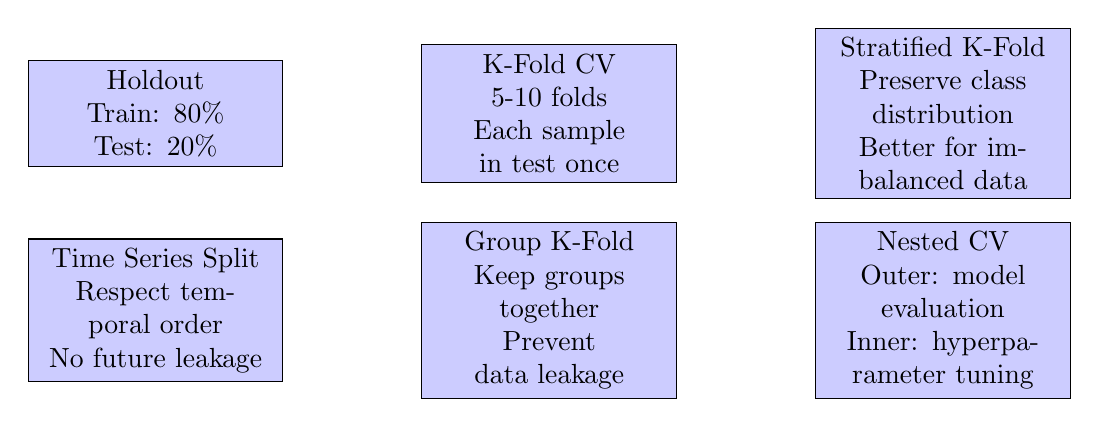
\begin{tikzpicture}[node distance=2cm]
    \tikzstyle{split} = [rectangle, draw, fill=blue!20, text width=3cm, text centered, minimum height=0.8cm]
    \tikzstyle{arrow} = [thick,->,>=stealth]

    % Holdout
    \node [split] (holdout) at (0,0) {Holdout\\Train: 80\%\\Test: 20\%};

    % K-Fold
    \node [split] (kfold) at (5,0) {K-Fold CV\\5-10 folds\\Each sample in test once};

    % Stratified K-Fold
    \node [split] (stratified) at (10,0) {Stratified K-Fold\\Preserve class distribution\\Better for imbalanced data};

    % Time series split
    \node [split] (timeseries) at (0,-2.5) {Time Series Split\\Respect temporal order\\No future leakage};

    % Group K-Fold
    \node [split] (group) at (5,-2.5) {Group K-Fold\\Keep groups together\\Prevent data leakage};

    % Nested CV
    \node [split] (nested) at (10,-2.5) {Nested CV\\Outer: model evaluation\\Inner: hyperparameter tuning};

\end{tikzpicture}
\caption{Model validation strategies for different scenarios}
\label{fig:validation_strategies}
\end{figure}

\begin{lstlisting}[style=python, caption=Comprehensive model validation framework]
from sklearn.model_selection import (
    cross_val_score, cross_validate,
    StratifiedKFold, TimeSeriesSplit, GroupKFold
)
from sklearn.metrics import (
    accuracy_score, precision_score, recall_score, f1_score,
    roc_auc_score, average_precision_score,
    confusion_matrix, classification_report
)
import pandas as pd
import numpy as np
from typing import Dict, List, Any
import warnings

class ModelValidator:
    """Comprehensive model validation framework"""

    def __init__(self, model, X, y, groups=None, is_timeseries=False):
        self.model = model
        self.X = X
        self.y = y
        self.groups = groups
        self.is_timeseries = is_timeseries

    def validate_comprehensive(self, cv_folds: int = 5) -> Dict[str, Any]:
        """Perform comprehensive validation with multiple metrics"""

        # Choose appropriate cross-validation strategy
        if self.is_timeseries:
            cv = TimeSeriesSplit(n_splits=cv_folds)
            cv_name = "TimeSeriesSplit"
        elif self.groups is not None:
            cv = GroupKFold(n_splits=cv_folds)
            cv_name = "GroupKFold"
        else:
            cv = StratifiedKFold(n_splits=cv_folds, shuffle=True, random_state=42)
            cv_name = "StratifiedKFold"

        # Define scoring metrics
        scoring = {
            'accuracy': 'accuracy',
            'precision': 'precision',
            'recall': 'recall',
            'f1': 'f1',
            'roc_auc': 'roc_auc',
            'average_precision': 'average_precision'
        }

        # Perform cross-validation
        cv_results = cross_validate(
            self.model,
            self.X,
            self.y,
            cv=cv,
            groups=self.groups,
            scoring=scoring,
            return_train_score=True,
            n_jobs=-1
        )

        # Aggregate results
        results = {
            'cv_strategy': cv_name,
            'cv_folds': cv_folds,
            'metrics': {}
        }

        for metric in scoring.keys():
            train_scores = cv_results[f'train_{metric}']
            test_scores = cv_results[f'test_{metric}']

            results['metrics'][metric] = {
                'train_mean': train_scores.mean(),
                'train_std': train_scores.std(),
                'test_mean': test_scores.mean(),
                'test_std': test_scores.std(),
                'overfitting': train_scores.mean() - test_scores.mean()
            }

        # Compute additional diagnostics
        results['diagnostics'] = self._compute_diagnostics(cv_results)

        return results

    def _compute_diagnostics(self, cv_results: Dict) -> Dict[str, float]:
        """Compute diagnostic metrics"""
        diagnostics = {}

        # Variance across folds (instability indicator)
        for metric in ['accuracy', 'precision', 'recall', 'f1']:
            test_scores = cv_results[f'test_{metric}']
            diagnostics[f'{metric}_variance'] = test_scores.var()

        # Overfitting ratio
        train_acc = cv_results['train_accuracy'].mean()
        test_acc = cv_results['test_accuracy'].mean()
        diagnostics['overfitting_ratio'] = train_acc / test_acc if test_acc > 0 else np.inf

        return diagnostics

    def learning_curve_analysis(self, train_sizes: List[float] = None):
        """Analyze learning curves to diagnose bias/variance"""
        from sklearn.model_selection import learning_curve
        import matplotlib.pyplot as plt

        if train_sizes is None:
            train_sizes = np.linspace(0.1, 1.0, 10)

        train_sizes_abs, train_scores, val_scores = learning_curve(
            self.model,
            self.X,
            self.y,
            train_sizes=train_sizes,
            cv=5,
            n_jobs=-1,
            scoring='accuracy'
        )

        # Plot learning curves
        plt.figure(figsize=(10, 6))
        plt.plot(train_sizes_abs, train_scores.mean(axis=1),
                label='Training score', marker='o')
        plt.plot(train_sizes_abs, val_scores.mean(axis=1),
                label='Validation score', marker='o')
        plt.fill_between(train_sizes_abs,
                        train_scores.mean(axis=1) - train_scores.std(axis=1),
                        train_scores.mean(axis=1) + train_scores.std(axis=1),
                        alpha=0.1)
        plt.fill_between(train_sizes_abs,
                        val_scores.mean(axis=1) - val_scores.std(axis=1),
                        val_scores.mean(axis=1) + val_scores.std(axis=1),
                        alpha=0.1)
        plt.xlabel('Training Examples')
        plt.ylabel('Accuracy')
        plt.title('Learning Curves')
        plt.legend()
        plt.grid(True)
        plt.savefig('learning_curves.png', dpi=300, bbox_inches='tight')
        plt.close()

        # Diagnose bias/variance
        final_train_score = train_scores.mean(axis=1)[-1]
        final_val_score = val_scores.mean(axis=1)[-1]
        gap = final_train_score - final_val_score

        diagnosis = {
            'final_train_score': final_train_score,
            'final_val_score': final_val_score,
            'train_val_gap': gap,
            'diagnosis': self._diagnose_bias_variance(final_train_score, final_val_score, gap)
        }

        return diagnosis

    def _diagnose_bias_variance(self, train_score, val_score, gap):
        """Diagnose bias/variance issues"""
        if train_score < 0.85 and val_score < 0.85:
            return "High Bias (Underfitting): Both scores are low. Try more complex model."
        elif gap > 0.1:
            return "High Variance (Overfitting): Large gap between scores. Try regularization, more data, or simpler model."
        elif train_score > 0.9 and val_score > 0.85 and gap < 0.05:
            return "Good Fit: Model is performing well."
        else:
            return "Moderate fit: Consider further tuning."

    def bootstrap_confidence_intervals(self, n_iterations: int = 1000, confidence: float = 0.95):
        """Compute bootstrap confidence intervals for metrics"""
        from sklearn.utils import resample

        bootstrap_scores = {
            'accuracy': [],
            'precision': [],
            'recall': [],
            'f1': []
        }

        for i in range(n_iterations):
            # Bootstrap sample
            X_boot, y_boot = resample(self.X, self.y, random_state=i)

            # Train on bootstrap sample
            self.model.fit(X_boot, y_boot)

            # Evaluate on out-of-bag samples
            oob_indices = list(set(range(len(self.X))) - set(X_boot.index))
            if len(oob_indices) > 0:
                X_oob = self.X.iloc[oob_indices]
                y_oob = self.y.iloc[oob_indices]

                y_pred = self.model.predict(X_oob)

                bootstrap_scores['accuracy'].append(accuracy_score(y_oob, y_pred))
                bootstrap_scores['precision'].append(precision_score(y_oob, y_pred, zero_division=0))
                bootstrap_scores['recall'].append(recall_score(y_oob, y_pred, zero_division=0))
                bootstrap_scores['f1'].append(f1_score(y_oob, y_pred, zero_division=0))

        # Compute confidence intervals
        alpha = 1 - confidence
        confidence_intervals = {}

        for metric, scores in bootstrap_scores.items():
            scores = np.array(scores)
            lower = np.percentile(scores, 100 * alpha / 2)
            upper = np.percentile(scores, 100 * (1 - alpha / 2))
            mean = scores.mean()

            confidence_intervals[metric] = {
                'mean': mean,
                'lower': lower,
                'upper': upper,
                'std': scores.std()
            }

        return confidence_intervals

    def statistical_significance_test(self, baseline_model, n_trials: int = 30):
        """Test if model is significantly better than baseline"""
        from scipy import stats

        model_scores = []
        baseline_scores = []

        for i in range(n_trials):
            # Split data
            from sklearn.model_selection import train_test_split
            X_train, X_test, y_train, y_test = train_test_split(
                self.X, self.y, test_size=0.2, random_state=i
            )

            # Train and evaluate both models
            self.model.fit(X_train, y_train)
            baseline_model.fit(X_train, y_train)

            model_scores.append(self.model.score(X_test, y_test))
            baseline_scores.append(baseline_model.score(X_test, y_test))

        # Paired t-test
        t_stat, p_value = stats.ttest_rel(model_scores, baseline_scores)

        # Effect size (Cohen's d)
        diff = np.array(model_scores) - np.array(baseline_scores)
        cohens_d = diff.mean() / diff.std()

        result = {
            'model_mean': np.mean(model_scores),
            'baseline_mean': np.mean(baseline_scores),
            'difference': np.mean(model_scores) - np.mean(baseline_scores),
            't_statistic': t_stat,
            'p_value': p_value,
            'cohens_d': cohens_d,
            'significant': p_value < 0.05,
            'interpretation': self._interpret_significance(p_value, cohens_d)
        }

        return result

    def _interpret_significance(self, p_value, cohens_d):
        """Interpret statistical significance results"""
        if p_value >= 0.05:
            return "No significant difference between models"
        elif abs(cohens_d) < 0.2:
            return "Statistically significant but small effect size"
        elif abs(cohens_d) < 0.5:
            return "Statistically significant with medium effect size"
        else:
            return "Statistically significant with large effect size"

# Usage example
if __name__ == '__main__':
    from sklearn.datasets import make_classification
    from sklearn.ensemble import RandomForestClassifier
    from sklearn.tree import DecisionTreeClassifier

    # Generate data
    X, y = make_classification(n_samples=1000, n_features=20, random_state=42)
    X = pd.DataFrame(X, columns=[f'feature_{i}' for i in range(20)])
    y = pd.Series(y)

    # Create validator
    model = RandomForestClassifier(n_estimators=100, random_state=42)
    validator = ModelValidator(model, X, y)

    # Comprehensive validation
    results = validator.validate_comprehensive(cv_folds=5)
    print("Cross-Validation Results:")
    for metric, values in results['metrics'].items():
        print(f"  {metric}:")
        print(f"    Test: {values['test_mean']:.4f} ± {values['test_std']:.4f}")
        print(f"    Train: {values['train_mean']:.4f} ± {values['train_std']:.4f}")
        print(f"    Overfitting: {values['overfitting']:.4f}")

    # Learning curves
    lc_results = validator.learning_curve_analysis()
    print(f"\nLearning Curve Diagnosis: {lc_results['diagnosis']}")

    # Bootstrap confidence intervals
    ci_results = validator.bootstrap_confidence_intervals(n_iterations=100)
    print("\nBootstrap Confidence Intervals (95%):")
    for metric, values in ci_results.items():
        print(f"  {metric}: {values['mean']:.4f} [{values['lower']:.4f}, {values['upper']:.4f}]")

    # Compare to baseline
    baseline = DecisionTreeClassifier(random_state=42)
    sig_test = validator.statistical_significance_test(baseline, n_trials=10)
    print(f"\nStatistical Significance Test:")
    print(f"  Model: {sig_test['model_mean']:.4f}")
    print(f"  Baseline: {sig_test['baseline_mean']:.4f}")
    print(f"  p-value: {sig_test['p_value']:.4f}")
    print(f"  {sig_test['interpretation']}")
\end{lstlisting}

\section{A/B Testing for ML Models}

A/B testing validates model improvements in production by comparing challenger models against the current champion.

\subsection{A/B Testing Framework}

\begin{figure}[h]
\centering
\begin{tikzpicture}[node distance=2.5cm, auto]
    \tikzstyle{component} = [rectangle, draw, fill=blue!20, text width=2.5cm, text centered, minimum height=1cm]
    \tikzstyle{decision} = [diamond, draw, fill=yellow!20, text width=2cm, text centered, minimum height=1.5cm]
    \tikzstyle{data} = [cylinder, draw, fill=green!20, text width=2cm, text centered, minimum height=1cm, shape aspect=0.3]
    \tikzstyle{arrow} = [thick,->,>=stealth]

    \node [component] (traffic) {Incoming Traffic};
    \node [decision, below of=traffic, node distance=2.5cm] (split) {Traffic Splitter};
    \node [component, below left of=split, node distance=3cm] (control) {Model A\\(Control)};
    \node [component, below right of=split, node distance=3cm] (treatment) {Model B\\(Treatment)};
    \node [data, below of=control, node distance=2.5cm, xshift=3cm] (metrics) {Metrics Collection};
    \node [decision, below of=metrics, node distance=2.5cm] (analysis) {Statistical Analysis};
    \node [component, below of=analysis, node distance=2.5cm] (decision_node) {Promotion Decision};

    \draw [arrow] (traffic) -- (split);
    \draw [arrow] (split) -- (control) node[midway, left] {50\%};
    \draw [arrow] (split) -- (treatment) node[midway, right] {50\%};
    \draw [arrow] (control) -- (metrics);
    \draw [arrow] (treatment) -- (metrics);
    \draw [arrow] (metrics) -- (analysis);
    \draw [arrow] (analysis) -- (decision_node);
\end{tikzpicture}
\caption{A/B testing framework for ML models}
\label{fig:ab_testing}
\end{figure}

\begin{lstlisting}[style=python, caption=Production A/B testing framework for ML models]
from dataclasses import dataclass
from typing import Dict, List, Callable, Any
import numpy as np
import pandas as pd
from scipy import stats
from datetime import datetime, timedelta
import hashlib

@dataclass
class ABTestConfig:
    """Configuration for A/B test"""
    test_name: str
    control_model_id: str
    treatment_model_id: str
    traffic_split: float = 0.5
    min_sample_size: int = 1000
    min_duration_days: int = 7
    significance_level: float = 0.05
    metrics: List[str] = None

class ABTestManager:
    """Manage A/B tests for ML models"""

    def __init__(self, config: ABTestConfig):
        self.config = config
        self.assignments = {}  # user_id -> variant
        self.results = {'control': [], 'treatment': []}
        self.start_time = datetime.now()

    def assign_variant(self, user_id: str) -> str:
        """Assign user to variant using consistent hashing"""
        # Check if user already assigned
        if user_id in self.assignments:
            return self.assignments[user_id]

        # Hash user ID for consistent assignment
        hash_value = int(hashlib.md5(
            f"{user_id}{self.config.test_name}".encode()
        ).hexdigest(), 16)

        # Assign based on hash and traffic split
        if (hash_value % 100) / 100 < self.config.traffic_split:
            variant = 'control'
        else:
            variant = 'treatment'

        self.assignments[user_id] = variant
        return variant

    def get_model_for_user(self, user_id: str) -> str:
        """Get appropriate model ID for user"""
        variant = self.assign_variant(user_id)

        if variant == 'control':
            return self.config.control_model_id
        else:
            return self.config.treatment_model_id

    def log_result(self, user_id: str, metrics: Dict[str, float]):
        """Log result for user"""
        variant = self.assignments.get(user_id)
        if variant:
            self.results[variant].append({
                'user_id': user_id,
                'timestamp': datetime.now(),
                **metrics
            })

    def analyze_results(self) -> Dict[str, Any]:
        """Analyze A/B test results"""
        # Convert to DataFrames
        control_df = pd.DataFrame(self.results['control'])
        treatment_df = pd.DataFrame(self.results['treatment'])

        if len(control_df) < self.config.min_sample_size or \
           len(treatment_df) < self.config.min_sample_size:
            return {
                'status': 'insufficient_data',
                'control_samples': len(control_df),
                'treatment_samples': len(treatment_df),
                'required_samples': self.config.min_sample_size
            }

        # Check duration
        duration = datetime.now() - self.start_time
        if duration < timedelta(days=self.config.min_duration_days):
            return {
                'status': 'insufficient_duration',
                'current_duration_hours': duration.total_seconds() / 3600,
                'required_duration_hours': self.config.min_duration_days * 24
            }

        # Analyze each metric
        analysis_results = {
            'status': 'complete',
            'duration_days': duration.days,
            'control_samples': len(control_df),
            'treatment_samples': len(treatment_df),
            'metrics': {}
        }

        for metric in self.config.metrics:
            control_values = control_df[metric].values
            treatment_values = treatment_df[metric].values

            metric_analysis = self._analyze_metric(
                metric,
                control_values,
                treatment_values
            )

            analysis_results['metrics'][metric] = metric_analysis

        # Overall recommendation
        analysis_results['recommendation'] = self._make_recommendation(
            analysis_results['metrics']
        )

        return analysis_results

    def _analyze_metric(self, metric_name: str,
                       control: np.ndarray,
                       treatment: np.ndarray) -> Dict[str, Any]:
        """Analyze single metric"""
        # Descriptive statistics
        control_mean = control.mean()
        treatment_mean = treatment.mean()
        lift = (treatment_mean - control_mean) / control_mean if control_mean != 0 else 0

        # Statistical test
        t_stat, p_value = stats.ttest_ind(treatment, control)

        # Effect size (Cohen's d)
        pooled_std = np.sqrt((control.var() + treatment.var()) / 2)
        cohens_d = (treatment_mean - control_mean) / pooled_std if pooled_std != 0 else 0

        # Confidence interval for difference
        se_diff = np.sqrt(control.var()/len(control) + treatment.var()/len(treatment))
        ci_lower = (treatment_mean - control_mean) - 1.96 * se_diff
        ci_upper = (treatment_mean - control_mean) + 1.96 * se_diff

        # Power analysis
        power = self._compute_power(control, treatment, self.config.significance_level)

        return {
            'control_mean': control_mean,
            'control_std': control.std(),
            'treatment_mean': treatment_mean,
            'treatment_std': treatment.std(),
            'lift_percent': lift * 100,
            'absolute_difference': treatment_mean - control_mean,
            'ci_lower': ci_lower,
            'ci_upper': ci_upper,
            'p_value': p_value,
            'cohens_d': cohens_d,
            'power': power,
            'significant': p_value < self.config.significance_level,
            'interpretation': self._interpret_result(p_value, lift, cohens_d, power)
        }

    def _compute_power(self, control, treatment, alpha):
        """Compute statistical power"""
        from statsmodels.stats.power import ttest_power

        effect_size = (treatment.mean() - control.mean()) / np.sqrt(
            (control.var() + treatment.var()) / 2
        )

        nobs = min(len(control), len(treatment))

        try:
            power = ttest_power(
                effect_size,
                nobs=nobs,
                alpha=alpha,
                alternative='two-sided'
            )
            return power
        except:
            return None

    def _interpret_result(self, p_value, lift, cohens_d, power):
        """Interpret test results"""
        if p_value >= self.config.significance_level:
            return "No significant difference detected"

        if power and power < 0.8:
            return "Significant but underpowered - consider longer test"

        if abs(cohens_d) < 0.2:
            return f"Significant with {lift*100:.2f}% lift but small effect size"
        elif abs(cohens_d) < 0.5:
            return f"Significant with {lift*100:.2f}% lift and medium effect size"
        else:
            return f"Significant with {lift*100:.2f}% lift and large effect size"

    def _make_recommendation(self, metrics_analysis: Dict) -> str:
        """Make overall recommendation based on all metrics"""
        primary_metric = self.config.metrics[0]
        primary_result = metrics_analysis[primary_metric]

        if not primary_result['significant']:
            return "KEEP CONTROL: No significant improvement in primary metric"

        if primary_result['lift_percent'] < 0:
            return "KEEP CONTROL: Treatment performed worse"

        # Check if all metrics improved or stayed neutral
        all_positive = all(
            m['lift_percent'] >= 0 or not m['significant']
            for m in metrics_analysis.values()
        )

        if not all_positive:
            return "CAUTIOUS ROLLOUT: Primary improved but some metrics degraded"

        # Check power
        if primary_result.get('power') and primary_result['power'] < 0.8:
            return "EXTEND TEST: Results promising but underpowered"

        return f"PROMOTE TREATMENT: Significant improvement of {primary_result['lift_percent']:.2f}%"

    def sequential_analysis(self, alpha_spending: str = 'obrien_fleming'):
        """Perform sequential analysis for early stopping"""
        from statsmodels.stats.multitest import multipletests

        # This is a simplified sequential testing approach
        # Production systems should use proper sequential testing frameworks

        control_df = pd.DataFrame(self.results['control'])
        treatment_df = pd.DataFrame(self.results['treatment'])

        if len(control_df) < 100 or len(treatment_df) < 100:
            return {'decision': 'continue', 'reason': 'Insufficient data for interim analysis'}

        # Run interim analysis
        interim_results = self.analyze_results()

        if interim_results['status'] != 'complete':
            return {'decision': 'continue', 'reason': interim_results['status']}

        primary_metric = self.config.metrics[0]
        p_value = interim_results['metrics'][primary_metric]['p_value']

        # Adjust significance level for interim analysis (Bonferroni correction)
        # In practice, use more sophisticated methods like O'Brien-Fleming
        adjusted_alpha = self.config.significance_level / 5  # Assume max 5 interim analyses

        if p_value < adjusted_alpha and interim_results['metrics'][primary_metric]['lift_percent'] > 5:
            return {
                'decision': 'stop_early_treatment_wins',
                'reason': f"Strong evidence for treatment (p={p_value:.4f})"
            }
        elif p_value < adjusted_alpha and interim_results['metrics'][primary_metric]['lift_percent'] < -5:
            return {
                'decision': 'stop_early_control_wins',
                'reason': f"Treatment performs worse (p={p_value:.4f})"
            }
        else:
            return {'decision': 'continue', 'reason': 'Inconclusive interim results'}

# Usage example
if __name__ == '__main__':
    # Configure A/B test
    config = ABTestConfig(
        test_name='model_v2_test',
        control_model_id='model_v1',
        treatment_model_id='model_v2',
        traffic_split=0.5,
        min_sample_size=1000,
        min_duration_days=7,
        metrics=['ctr', 'conversion_rate', 'revenue']
    )

    ab_test = ABTestManager(config)

    # Simulate user interactions
    np.random.seed(42)
    for user_id in range(3000):
        user_id_str = f'user_{user_id}'

        # Get model assignment
        model_id = ab_test.get_model_for_user(user_id_str)

        # Simulate metrics (treatment slightly better)
        if model_id == 'model_v1':
            metrics = {
                'ctr': np.random.binomial(1, 0.10),
                'conversion_rate': np.random.binomial(1, 0.05),
                'revenue': np.random.exponential(10) if np.random.random() < 0.05 else 0
            }
        else:
            metrics = {
                'ctr': np.random.binomial(1, 0.12),  # 20% relative lift
                'conversion_rate': np.random.binomial(1, 0.055),  # 10% relative lift
                'revenue': np.random.exponential(11) if np.random.random() < 0.055 else 0
            }

        ab_test.log_result(user_id_str, metrics)

    # Analyze results
    results = ab_test.analyze_results()

    print(f"Status: {results['status']}")
    print(f"Duration: {results.get('duration_days', 0)} days")
    print(f"\nResults:")
    for metric, analysis in results.get('metrics', {}).items():
        print(f"\n{metric}:")
        print(f"  Control: {analysis['control_mean']:.4f} ± {analysis['control_std']:.4f}")
        print(f"  Treatment: {analysis['treatment_mean']:.4f} ± {analysis['treatment_std']:.4f}")
        print(f"  Lift: {analysis['lift_percent']:.2f}%")
        print(f"  p-value: {analysis['p_value']:.4f}")
        print(f"  Significant: {analysis['significant']}")
        print(f"  {analysis['interpretation']}")

    print(f"\n{results.get('recommendation', 'No recommendation yet')}")
\end{lstlisting}

\section{BigQuery ML ARIMA\_PLUS Case Study}

This case study demonstrates end-to-end ML pipeline design using BigQuery ML for time series forecasting with automated model selection and evaluation.

\subsection{Problem: Sales Forecasting}

A retail company needs to forecast daily sales for inventory planning. The pipeline must:
\begin{itemize}
    \item Train models weekly on historical sales data
    \item Evaluate forecast accuracy automatically
    \item Deploy best models to production
    \item Monitor model drift and retrain when needed
\end{itemize}

\begin{lstlisting}[style=python, caption=BigQuery ML ARIMA\_PLUS automated forecasting pipeline]
from google.cloud import bigquery
from google.cloud.bigquery import ScalarQueryParameter
import pandas as pd
from datetime import datetime, timedelta
import mlflow

class BigQueryMLPipeline:
    """Production pipeline for BigQuery ML ARIMA_PLUS forecasting"""

    def __init__(self, project_id: str, dataset_id: str):
        self.client = bigquery.Client(project=project_id)
        self.project_id = project_id
        self.dataset_id = dataset_id
        self.model_name = "sales_forecast_model"

    def create_training_data(self, start_date: str, end_date: str):
        """Prepare time series data for training"""
        query = f"""
        CREATE OR REPLACE TABLE `{self.project_id}.{self.dataset_id}.training_data` AS
        SELECT
            DATE(timestamp) as date,
            SUM(sales) as total_sales,
            AVG(temperature) as avg_temperature,
            MAX(is_holiday) as is_holiday,
            MAX(is_weekend) as is_weekend
        FROM `{self.project_id}.{self.dataset_id}.raw_sales`
        WHERE DATE(timestamp) BETWEEN @start_date AND @end_date
        GROUP BY DATE(timestamp)
        ORDER BY date
        """

        job_config = bigquery.QueryJobConfig(
            query_parameters=[
                ScalarQueryParameter("start_date", "DATE", start_date),
                ScalarQueryParameter("end_date", "DATE", end_date),
            ]
        )

        query_job = self.client.query(query, job_config=job_config)
        query_job.result()

        print(f"Training data created: {start_date} to {end_date}")

    def train_arima_model(self):
        """Train ARIMA_PLUS model with auto parameter selection"""
        query = f"""
        CREATE OR REPLACE MODEL `{self.project_id}.{self.dataset_id}.{self.model_name}`
        OPTIONS(
            model_type='ARIMA_PLUS',
            time_series_timestamp_col='date',
            time_series_data_col='total_sales',
            time_series_id_col=NULL,
            holiday_region='US',
            data_frequency='AUTO_FREQUENCY',

            -- Include additional regressors
            include_drift=TRUE,
            clean_spikes_and_dips=TRUE,
            adjust_step_changes=TRUE,

            -- Auto parameter selection
            auto_arima=TRUE,
            auto_arima_max_order=5,

            -- Model evaluation
            decompose_time_series=TRUE
        ) AS
        SELECT
            date,
            total_sales,
            avg_temperature,
            is_holiday,
            is_weekend
        FROM `{self.project_id}.{self.dataset_id}.training_data`
        """

        query_job = self.client.query(query)
        query_job.result()

        print(f"ARIMA_PLUS model trained: {self.model_name}")

    def evaluate_model(self) -> pd.DataFrame:
        """Evaluate model performance"""
        # Get training metrics
        metrics_query = f"""
        SELECT
            *
        FROM ML.ARIMA_EVALUATE(
            MODEL `{self.project_id}.{self.dataset_id}.{self.model_name}`
        )
        """

        metrics_df = self.client.query(metrics_query).to_dataframe()

        # Get detailed evaluation
        eval_query = f"""
        SELECT
            *
        FROM ML.EVALUATE(
            MODEL `{self.project_id}.{self.dataset_id}.{self.model_name}`,
            (
                SELECT
                    date,
                    total_sales,
                    avg_temperature,
                    is_holiday,
                    is_weekend
                FROM `{self.project_id}.{self.dataset_id}.training_data`
                ORDER BY date DESC
                LIMIT 30  -- Last 30 days for validation
            )
        )
        """

        eval_df = self.client.query(eval_query).to_dataframe()

        return {
            'arima_metrics': metrics_df,
            'evaluation': eval_df
        }

    def get_model_coefficients(self) -> pd.DataFrame:
        """Extract model coefficients and parameters"""
        query = f"""
        SELECT
            *
        FROM ML.ARIMA_COEFFICIENTS(
            MODEL `{self.project_id}.{self.dataset_id}.{self.model_name}`
        )
        """

        return self.client.query(query).to_dataframe()

    def forecast(self, horizon: int = 30, confidence_level: float = 0.95):
        """Generate forecasts with confidence intervals"""
        query = f"""
        SELECT
            *
        FROM ML.FORECAST(
            MODEL `{self.project_id}.{self.dataset_id}.{self.model_name}`,
            STRUCT(
                {horizon} AS horizon,
                {confidence_level} AS confidence_level
            )
        )
        """

        forecast_df = self.client.query(query).to_dataframe()

        # Save forecast to table
        table_id = f"{self.project_id}.{self.dataset_id}.forecasts"

        forecast_df['forecast_timestamp'] = datetime.now()
        forecast_df['model_name'] = self.model_name

        job_config = bigquery.LoadJobConfig(
            write_disposition=bigquery.WriteDisposition.WRITE_APPEND
        )

        self.client.load_table_from_dataframe(
            forecast_df, table_id, job_config=job_config
        ).result()

        return forecast_df

    def detect_anomalies(self, threshold: float = 0.95):
        """Detect anomalies in time series"""
        query = f"""
        SELECT
            *
        FROM ML.DETECT_ANOMALIES(
            MODEL `{self.project_id}.{self.dataset_id}.{self.model_name}`,
            STRUCT(
                {threshold} AS anomaly_prob_threshold
            ),
            (
                SELECT
                    date,
                    total_sales,
                    avg_temperature,
                    is_holiday,
                    is_weekend
                FROM `{self.project_id}.{self.dataset_id}.training_data`
                ORDER BY date DESC
                LIMIT 90  -- Last 90 days
            )
        )
        """

        anomalies_df = self.client.query(query).to_dataframe()
        return anomalies_df

    def explain_forecast(self, forecast_date: str):
        """Explain forecast using feature attributions"""
        query = f"""
        SELECT
            *
        FROM ML.EXPLAIN_FORECAST(
            MODEL `{self.project_id}.{self.dataset_id}.{self.model_name}`,
            STRUCT(
                30 AS horizon,
                0.95 AS confidence_level
            )
        )
        WHERE forecast_timestamp = @forecast_date
        """

        job_config = bigquery.QueryJobConfig(
            query_parameters=[
                ScalarQueryParameter("forecast_date", "DATE", forecast_date),
            ]
        )

        explanation_df = self.client.query(query, job_config=job_config).to_dataframe()
        return explanation_df

    def run_pipeline(self, train_start: str, train_end: str,
                    forecast_horizon: int = 30):
        """Execute complete pipeline"""
        print("=" * 60)
        print("BigQuery ML ARIMA_PLUS Forecasting Pipeline")
        print("=" * 60)

        # MLflow tracking
        mlflow.set_experiment("bigquery_ml_forecasting")

        with mlflow.start_run(run_name=f"arima_plus_{datetime.now().strftime('%Y%m%d')}"):
            # Log parameters
            mlflow.log_param("train_start", train_start)
            mlflow.log_param("train_end", train_end)
            mlflow.log_param("forecast_horizon", forecast_horizon)
            mlflow.log_param("model_type", "ARIMA_PLUS")

            # Step 1: Create training data
            print("\n1. Creating training data...")
            self.create_training_data(train_start, train_end)

            # Step 2: Train model
            print("\n2. Training ARIMA_PLUS model...")
            self.train_arima_model()

            # Step 3: Evaluate model
            print("\n3. Evaluating model...")
            evaluation = self.evaluate_model()

            # Log metrics
            arima_metrics = evaluation['arima_metrics'].iloc[0]
            mlflow.log_metric("AIC", arima_metrics.get('AIC', 0))
            mlflow.log_metric("variance", arima_metrics.get('variance', 0))

            if 'mean_absolute_error' in evaluation['evaluation'].columns:
                mae = evaluation['evaluation']['mean_absolute_error'].iloc[0]
                mlflow.log_metric("MAE", mae)

            print(f"\nModel Metrics:")
            print(evaluation['arima_metrics'])

            # Step 4: Get model details
            print("\n4. Extracting model coefficients...")
            coefficients = self.get_model_coefficients()
            print(coefficients)

            # Step 5: Generate forecast
            print(f"\n5. Generating {forecast_horizon}-day forecast...")
            forecast = self.forecast(horizon=forecast_horizon)
            print(f"Forecast generated for {len(forecast)} time steps")

            # Log forecast sample
            mlflow.log_text(
                forecast.head(10).to_string(),
                "forecast_sample.txt"
            )

            # Step 6: Detect anomalies
            print("\n6. Detecting anomalies...")
            anomalies = self.detect_anomalies()
            num_anomalies = len(anomalies[anomalies['is_anomaly'] == True])
            print(f"Detected {num_anomalies} anomalies in last 90 days")

            mlflow.log_metric("num_anomalies", num_anomalies)

            print("\n" + "=" * 60)
            print("Pipeline completed successfully!")
            print("=" * 60)

            return {
                'evaluation': evaluation,
                'coefficients': coefficients,
                'forecast': forecast,
                'anomalies': anomalies
            }

# Airflow DAG for automated execution
from airflow import DAG
from airflow.operators.python import PythonOperator
from airflow.utils.dates import days_ago
from datetime import timedelta

default_args = {
    'owner': 'ml_team',
    'depends_on_past': False,
    'email_on_failure': True,
    'email': ['ml-alerts@company.com'],
    'retries': 2,
    'retry_delay': timedelta(minutes=5),
}

def run_bigquery_ml_pipeline(**context):
    """Airflow task to run BigQuery ML pipeline"""
    execution_date = context['execution_date']

    # Training window: last 365 days before execution date
    train_end = execution_date.date()
    train_start = train_end - timedelta(days=365)

    # Initialize pipeline
    pipeline = BigQueryMLPipeline(
        project_id='my-project',
        dataset_id='sales_forecasting'
    )

    # Run pipeline
    results = pipeline.run_pipeline(
        train_start=train_start.isoformat(),
        train_end=train_end.isoformat(),
        forecast_horizon=30
    )

    # Push key metrics to XCom
    context['task_instance'].xcom_push(
        key='num_anomalies',
        value=len(results['anomalies'][results['anomalies']['is_anomaly'] == True])
    )

with DAG(
    'bigquery_ml_forecasting',
    default_args=default_args,
    description='Weekly sales forecasting with BigQuery ML',
    schedule_interval='0 2 * * 0',  # Weekly on Sunday
    start_date=days_ago(1),
    catchup=False,
    tags=['ml', 'forecasting', 'bigquery']
) as dag:

    forecast_task = PythonOperator(
        task_id='run_arima_forecast',
        python_callable=run_bigquery_ml_pipeline,
        provide_context=True,
        execution_timeout=timedelta(hours=2)
    )

# Usage example
if __name__ == '__main__':
    pipeline = BigQueryMLPipeline(
        project_id='my-project',
        dataset_id='sales_forecasting'
    )

    results = pipeline.run_pipeline(
        train_start='2023-01-01',
        train_end='2024-01-01',
        forecast_horizon=30
    )

    print("\nForecast Preview:")
    print(results['forecast'][['forecast_timestamp', 'forecast_value',
                               'standard_error', 'confidence_level']].head())
\end{lstlisting}

\section{Failure Handling and Retry Mechanisms}

Production pipelines must handle failures gracefully with appropriate retry strategies and circuit breakers.

\begin{lstlisting}[style=python, caption=Robust failure handling for ML pipelines]
from functools import wraps
import time
import logging
from typing import Callable, Any
from enum import Enum

logger = logging.getLogger(__name__)

class RetryStrategy(Enum):
    """Retry strategy types"""
    EXPONENTIAL_BACKOFF = "exponential"
    LINEAR_BACKOFF = "linear"
    FIXED_DELAY = "fixed"

class CircuitBreaker:
    """Circuit breaker pattern for external service calls"""

    def __init__(self, failure_threshold: int = 5, timeout: int = 60):
        self.failure_threshold = failure_threshold
        self.timeout = timeout
        self.failure_count = 0
        self.last_failure_time = None
        self.state = "CLOSED"  # CLOSED, OPEN, HALF_OPEN

    def call(self, func: Callable, *args, **kwargs) -> Any:
        """Execute function with circuit breaker"""
        if self.state == "OPEN":
            if time.time() - self.last_failure_time > self.timeout:
                self.state = "HALF_OPEN"
                logger.info("Circuit breaker entering HALF_OPEN state")
            else:
                raise Exception(f"Circuit breaker OPEN - service unavailable")

        try:
            result = func(*args, **kwargs)

            if self.state == "HALF_OPEN":
                self.state = "CLOSED"
                self.failure_count = 0
                logger.info("Circuit breaker reset to CLOSED")

            return result

        except Exception as e:
            self.failure_count += 1
            self.last_failure_time = time.time()

            if self.failure_count >= self.failure_threshold:
                self.state = "OPEN"
                logger.error(f"Circuit breaker opened after {self.failure_count} failures")

            raise

def retry_with_backoff(
    max_attempts: int = 3,
    strategy: RetryStrategy = RetryStrategy.EXPONENTIAL_BACKOFF,
    base_delay: float = 1.0,
    max_delay: float = 60.0,
    exceptions: tuple = (Exception,),
    on_retry: Callable = None
):
    """Decorator for retry with configurable backoff strategy"""

    def decorator(func):
        @wraps(func)
        def wrapper(*args, **kwargs):
            attempt = 0
            last_exception = None

            while attempt < max_attempts:
                try:
                    return func(*args, **kwargs)

                except exceptions as e:
                    attempt += 1
                    last_exception = e

                    if attempt >= max_attempts:
                        logger.error(
                            f"Function {func.__name__} failed after {max_attempts} attempts"
                        )
                        raise

                    # Calculate delay
                    if strategy == RetryStrategy.EXPONENTIAL_BACKOFF:
                        delay = min(base_delay * (2 ** (attempt - 1)), max_delay)
                    elif strategy == RetryStrategy.LINEAR_BACKOFF:
                        delay = min(base_delay * attempt, max_delay)
                    else:  # FIXED_DELAY
                        delay = base_delay

                    logger.warning(
                        f"Attempt {attempt}/{max_attempts} failed for {func.__name__}: {e}. "
                        f"Retrying in {delay:.2f}s..."
                    )

                    # Call retry callback if provided
                    if on_retry:
                        on_retry(attempt, delay, e)

                    time.sleep(delay)

            raise last_exception

        return wrapper
    return decorator

# Usage in pipeline tasks
@retry_with_backoff(
    max_attempts=3,
    strategy=RetryStrategy.EXPONENTIAL_BACKOFF,
    base_delay=1.0,
    exceptions=(ConnectionError, TimeoutError)
)
def fetch_training_data():
    """Fetch data with automatic retry"""
    # Implementation with potential network failures
    pass

# Circuit breaker usage
model_service_breaker = CircuitBreaker(failure_threshold=5, timeout=60)

def call_model_service(data):
    """Call external model service with circuit breaker"""
    return model_service_breaker.call(
        _internal_service_call,
        data
    )

def _internal_service_call(data):
    # Actual service call implementation
    pass
\end{lstlisting}

\section{Chapter Summary}

This chapter covered comprehensive training pipeline design patterns:

\begin{itemize}
    \item \textbf{Pipeline Orchestration}: Airflow, Kubeflow Pipelines with production examples
    \item \textbf{Experiment Tracking}: MLflow integration for reproducibility and comparison
    \item \textbf{Hyperparameter Optimization}: Optuna-based Bayesian optimization at scale
    \item \textbf{Model Validation}: Statistical validation frameworks with bias/variance analysis
    \item \textbf{A/B Testing}: Production A/B testing framework with statistical rigor
    \item \textbf{BigQuery ML Case Study}: End-to-end ARIMA_PLUS forecasting pipeline
    \item \textbf{Failure Handling}: Retry mechanisms, circuit breakers, and error recovery
\end{itemize}

Key takeaways:
\begin{enumerate}
    \item Training pipelines require different orchestration than traditional software
    \item Experiment tracking is essential for reproducibility and debugging
    \item Hyperparameter optimization should be automated and integrated into pipelines
    \item Model validation must go beyond simple accuracy metrics
    \item A/B testing validates model improvements in production
    \item Failure handling is critical for production reliability
\end{enumerate}

\section{Exercises}

\begin{exercise}
\textbf{Design Complete Training Pipeline}

Design and implement an end-to-end training pipeline using Airflow that:
\begin{enumerate}
    \item Extracts data from a data warehouse
    \item Performs data validation with Great Expectations
    \item Trains multiple model types (RF, GBM, XGBoost)
    \item Logs all experiments to MLflow
    \item Selects best model based on validation metrics
    \item Deploys to a model registry only if quality thresholds are met
    \item Sends notifications on success/failure
\end{enumerate}

Include proper error handling, retries, and resource management.
\end{exercise}

\begin{exercise}
\textbf{Implement Experiment Tracking}

Create an experiment tracking system that:
\begin{itemize}
    \item Tracks code version (git commit), data version (hash), environment (packages)
    \item Logs all hyperparameters and metrics
    \item Creates comparison visualizations between experiments
    \item Identifies the best model for production
    \item Ensures full reproducibility
\end{itemize}

Test reproducibility by running the same experiment twice and verifying identical results.
\end{exercise}

\begin{exercise}
\textbf{Hyperparameter Optimization}

Implement hyperparameter optimization using Optuna that:
\begin{enumerate}
    \item Optimizes across multiple model types
    \item Uses early stopping to prune unpromising trials
    \item Integrates with MLflow for experiment tracking
    \item Creates visualization of the optimization process
    \item Computes parameter importance
\end{enumerate}

Target: Find optimal hyperparameters within 100 trials that beat baseline by >5\%.
\end{exercise}

\begin{exercise}
\textbf{Model Validation Framework}

Build a comprehensive validation framework that:
\begin{itemize}
    \item Implements k-fold cross-validation with appropriate strategy
    \item Generates learning curves to diagnose bias/variance
    \item Computes bootstrap confidence intervals for metrics
    \item Performs statistical significance testing vs baseline
    \item Creates detailed validation reports
\end{itemize}

Apply to a classification problem and interpret all diagnostic plots.
\end{exercise}

\begin{exercise}
\textbf{A/B Testing Framework}

Implement a production A/B testing framework:
\begin{enumerate}
    \item Assign users consistently to control/treatment via hashing
    \item Track multiple metrics (primary and guardrail metrics)
    \item Perform statistical analysis with proper significance testing
    \item Compute confidence intervals and effect sizes
    \item Provide actionable recommendations
\end{enumerate}

Simulate an A/B test and demonstrate when to promote treatment vs keep control.
\end{exercise}

\begin{exercise}
\textbf{BigQuery ML Pipeline}

Create a production forecasting pipeline using BigQuery ML:
\begin{itemize}
    \item Train ARIMA_PLUS models on time series data
    \item Evaluate model performance automatically
    \item Generate forecasts with confidence intervals
    \item Detect anomalies in recent data
    \item Explain forecasts with feature attributions
    \item Orchestrate with Airflow on a weekly schedule
\end{itemize}

Deploy to production and monitor forecast accuracy over time.
\end{exercise}

\begin{exercise}
\textbf{Failure Recovery Mechanisms}

Implement robust failure handling for ML pipelines:
\begin{enumerate}
    \item Retry decorator with exponential backoff
    \item Circuit breaker for external service calls
    \item Checkpoint mechanism for long-running training
    \item Dead letter queue for failed records
    \item Alerting system for critical failures
\end{enumerate}

Test by injecting failures and verifying proper recovery.
\end{exercise}

\begin{exercise}
\textbf{Pipeline-as-Code}

Convert an existing ML workflow to pipeline-as-code:
\begin{itemize}
    \item Define pipeline in Python/YAML
    \item Parameterize all configurations
    \item Version control pipeline definitions
    \item Implement CI/CD for pipeline deployments
    \item Create automated tests for pipeline components
\end{itemize}

Deploy the same pipeline to dev, staging, and production environments.
\end{exercise}
